\documentclass[simplex.tex]{subfiles}
% NO NEED TO INPUT PREAMBLES HERE
% packages are inherited; you can compile this on its own

\onlyinsubfile{
\title{NeuroData SIMPLEX Report: Subfile}
}

\begin{document}
\onlyinsubfile{
\maketitle
\thispagestyle{empty}

The following report documents the progress made by the labs of Randal~Burns and Joshua~T.~Vogelstein at Johns Hopkins University towards goals set by the DARPA SIMPLEX grant.

%%%% Table of Contents
\tableofcontents

%%%% Publications
\bibliographystyle{IEEEtran}
\begin{spacing}{0.5}
\section*{Publications, Presentations, and Talks}
\vspace{-20pt}
\nocite{*}
{\footnotesize	\bibliography{simplex}}
\end{spacing}
%%%% End Publications
}


\subsection{ndmg}

Through the use of AWS Batch, a cloud deployment script has been added to the pipeline which enables users to run the
pipeline in the cloud directly on data also stored in the cloud. This additional feature significantly lowers the
barrier to entry for use of the pipeline, and enables researchers to process and store their data without requiring
physical compute or data storage hardware or management expertise in house. Figure \ref{fig:ndmgcloud} shows an example
workflow that could be used by researchers performing a study.


\begin{figure}[h!]
\begin{cframed}
\centering
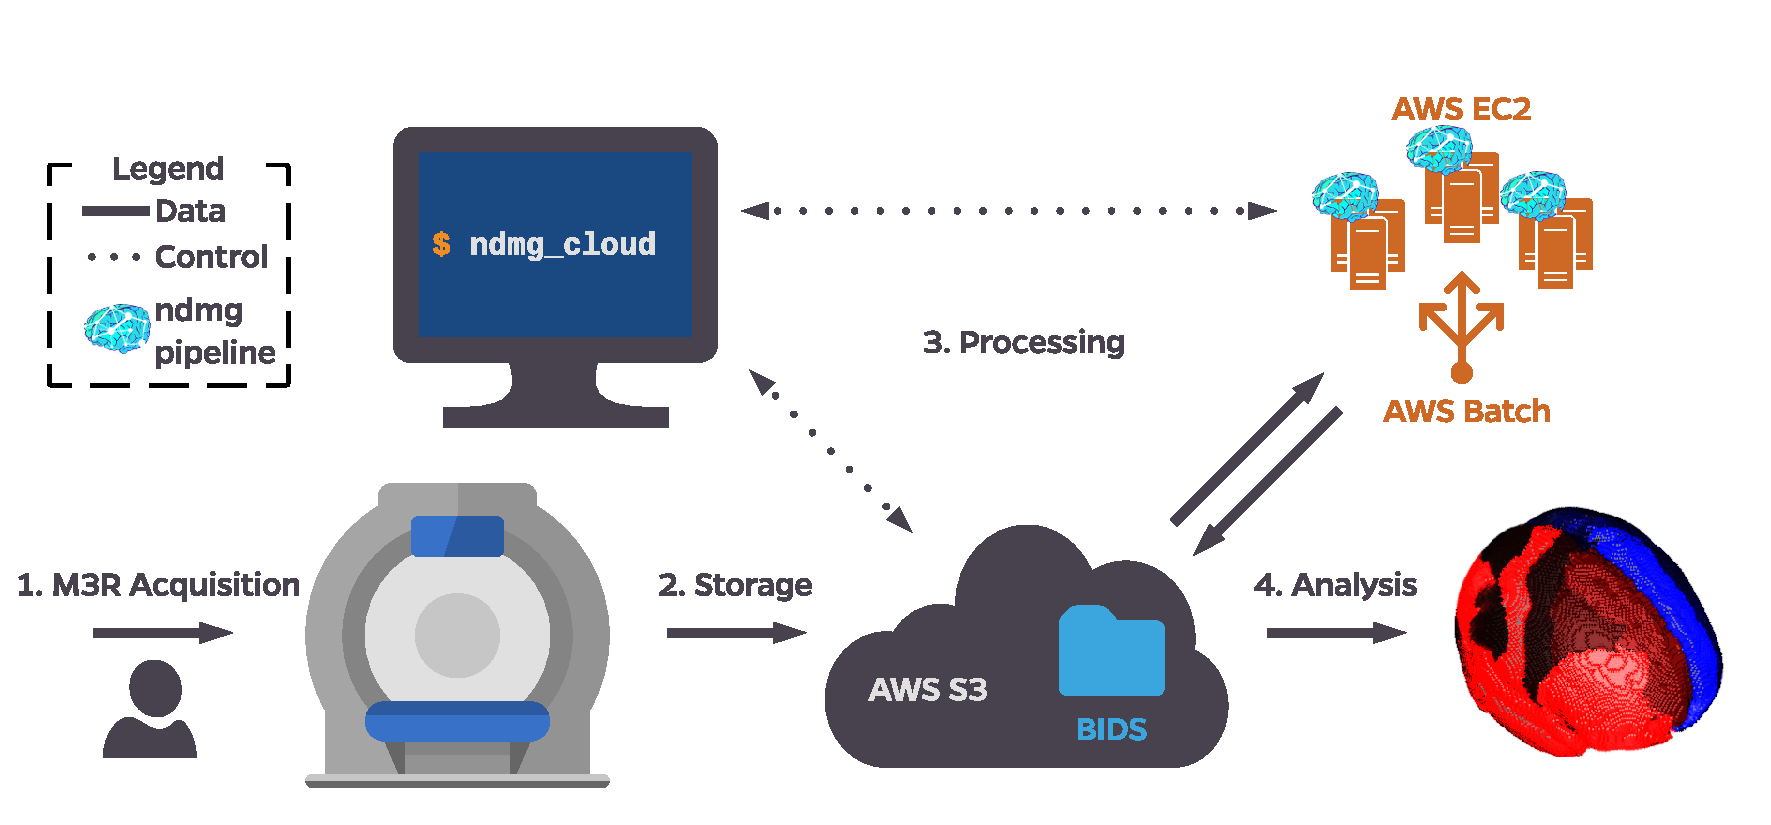
\includegraphics[width=0.95\textwidth]{../../figs/ndmgcloud.pdf}
\caption{\textbf{ndmg usage workflow}. The ndmg pipeline has been designed to minimize the technological equipment and
expertise required to go from raw imaging data to scientific analyses. Here we suggest an example workflow which
researchers can follow to accomplish this. After collecting multimodal MR (M3R) data for a study, the data can be
organized in accordance with the BIDS organization standard and stored in Amazon S3. Once in the cloud, through the use
of Amazon Batch and the ndmg pipeline's \texttt{ndmg\_cloud} routine, a series of parallel jobs can be launched which
process all of the uploaded data and return the derivatives to the cloud. Along with quality control figures and
measures, the derivatives are then retrievable by the researcher to perform further analysis.}
\label{fig:ndmgcloud}
\end{cframed}
\end{figure}
\end{document}
